\begin{frame}
	\frametitle{Weitere Optimierungen}
	\only<1,3,5> {
		\begin{itemize}
			\item<1->	$k$-opt-Verfahren.
			\item<3-> 	Ant-Colony-Optimization
			\item<5->	Andere Ansätze: Linear Programming
		\end{itemize}
	}

	\only<2> {
		\begin{figure}
			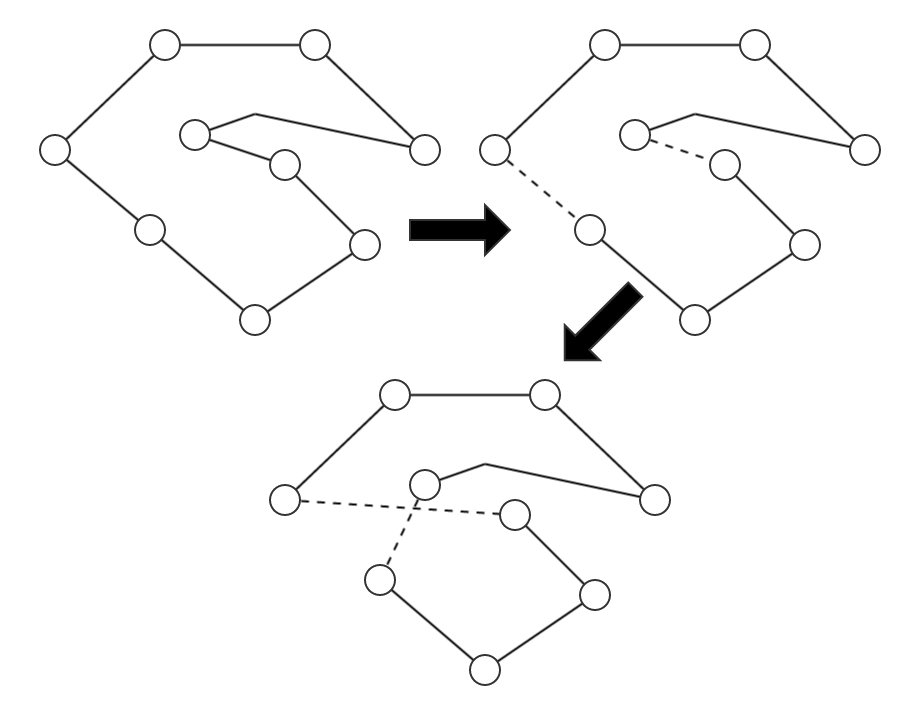
\includegraphics[scale=.2]{Showing_a_step_of_the_two-opt_heuristic.png}
			\caption{2-opt-Verfahren}
		\end{figure}
	}

	\only<4> 	{
		\begin{figure}
			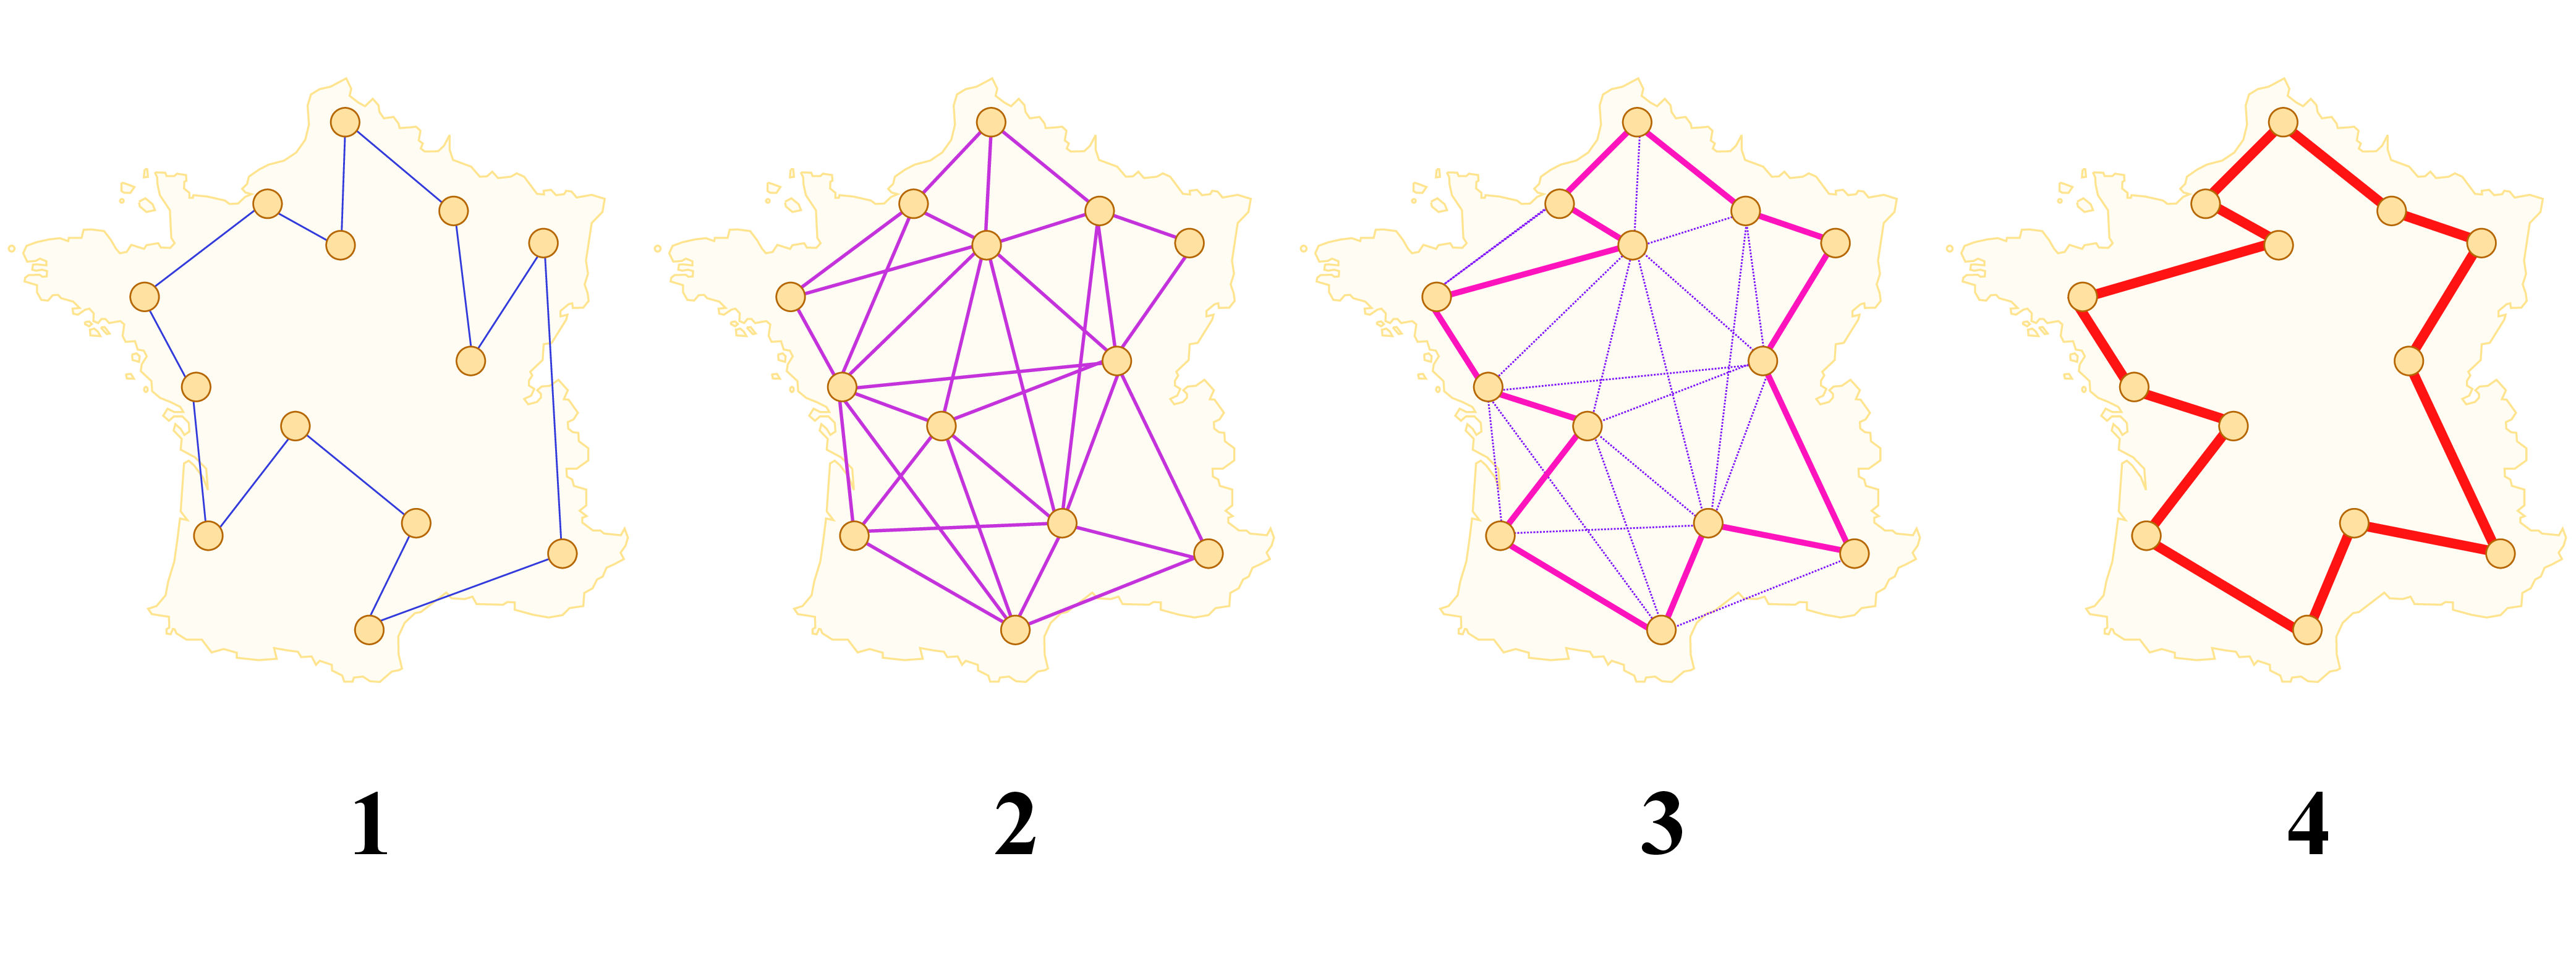
\includegraphics[scale=0.3]{images/traveling-salesman-problem}
			\caption{Die Dicke der Kanten ist proportional zu den Pheromonen, die darauf verteilt sind}
		\end{figure}
	}
\end{frame}